\documentclass{beamer}
\usefonttheme{serif}
\usepackage{biblatex}
\usepackage{textcomp}
\usepackage{wrapfig}

\addtobeamertemplate{navigation symbols}{}{%
    \usebeamerfont{footline}%
    \usebeamercolor[fg]{footline}%
    \hspace{1em}%
    \insertframenumber/\inserttotalframenumber
}
\setbeamercolor{footline}{fg=blue}
\setbeamerfont{footline}{series=\bfseries}


\title{Orientation Decoding at multiple resolutions at 7T}
\author{Ayan Sengupta\inst{1}}
\institute[Affiliations] % (optional)
{
  \inst{1}%
  Institute of Experimental Psychology\\
  Otto-von-Guericke University\\
  Magdeburg
  %~ \and
  %~ \inst{2}%
  %~ Institute of Theoretical Philosophy\\
  %~ University There
}
\logo{
\includegraphics[height=0.3cm]{../pictures/logo}\hfill}
\date{\today}




\begin{document}
\frame{\titlepage}
  \begin{frame}
    \frametitle{Orientation Decoding in primary visual cortex (V1)}
    \begin{center}
        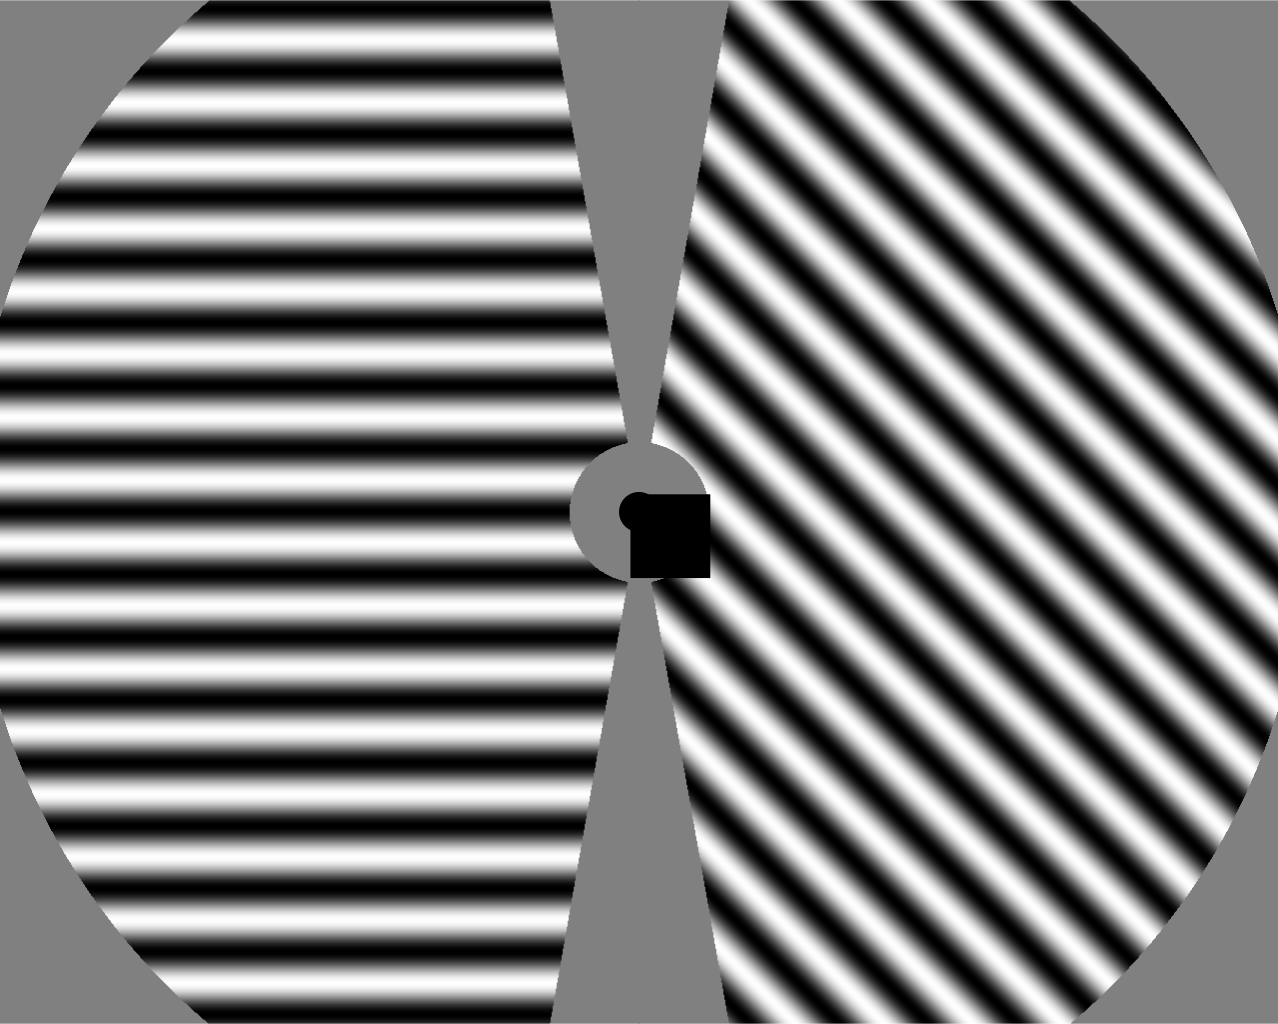
\includegraphics[height=5cm]{../pictures/exp_frame}
    \end{center}
    \begin{itemize}
        \item Most extensively studied paradigm.
        \item Important studies like Kamitani and Tong (2005), Haynes and Rees (2005),
        Swisher et al., (2010), Alink et al., (2013) etc.
        %~ \item Reliable Orientation Decoding from:
            %~ \begin{itemize}
                %~ \item 3 mm isotropic voxels (Kamitani and Tong, 2005)
                %~ \item 2 mm isotropic voxels (Alink et al., 2013)
                %~ \item 1 mm isotropic voxels (Swisher et al., 2010)
            %~ \end{itemize}
    \end{itemize}
    %Content goes here
  \end{frame}
    \begin{frame}
        \frametitle{Stimulus}
            \begin{center}
                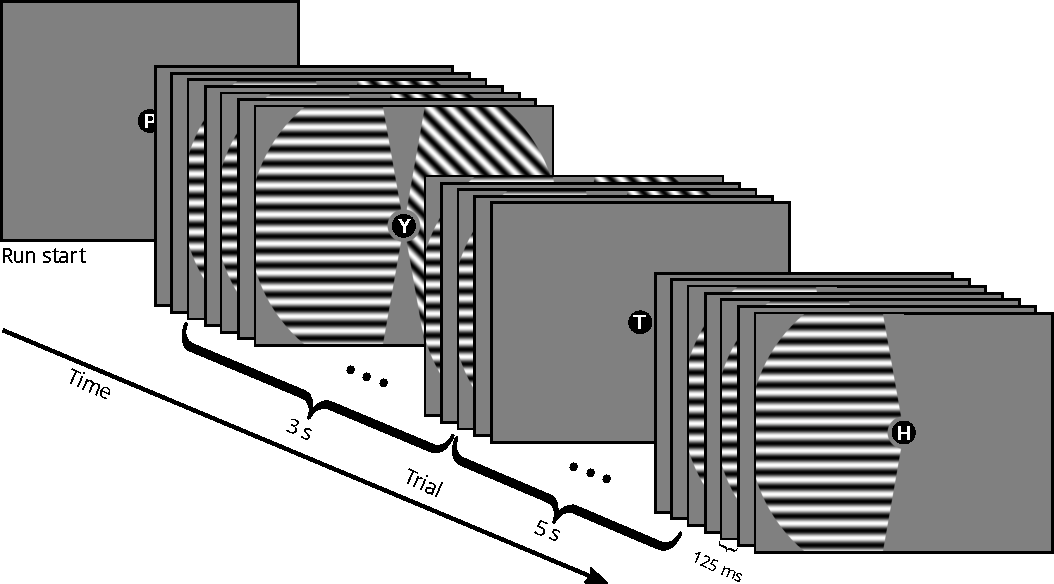
\includegraphics[height=4cm]{../pictures/stimulus}
            \end{center}
            \begin{itemize}
                \item 30 Trials = 1 Experimental run
                \item Number of runs = 10
                \item Total scan time = 40min
                \item 4 orientations in each hemifield (0\textdegree, 45\textdegree, 90\textdegree \& 135\textdegree) with random phase shifts
            \end{itemize}

    \end{frame}
 
  \begin{frame}
    \frametitle{General Workflow of Orientation decoding analysis}
        \begin{itemize}
            \item EPI acquisition in one particular resolution
            \item Volumetric Gaussian filtering with increase in kernel width (expressed in FWHM)
            \item Within-subject leave-one-run-out cross-validation with LinearSVM classifier
            \item Conclusion about the spatial scale of the Orientation specific signals 
        \end{itemize}  
    \end{frame}

  %~ \begin{frame}
    %~ \frametitle{High field fMRI unveils orientation columns in humans}
        %~ \begin{center}
            %~ 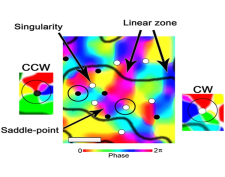
\includegraphics[height=4cm]{../pictures/Yacoub_pinwheel}
        %~ \end{center}
        %~ \begin{itemize}
            %~ \item Yacoub et al. (2008) used high field strength (7T)
            %~ \item Voxel dimensions - 0.5mm x 0.5mm x 3.0mm
            %~ \item The pinwheel pattern maps were reproducible
        %~ \end{itemize}  
    %~ \end{frame}
%~ 
  %~ \begin{frame}
    %~ \frametitle{Impressions about Optimal Acquisition Resolution}
        %~ \begin{itemize}
            %~ \item Smaller the voxel size = Better Orientation Signals from the Orientation Columns
            %~ \item If sub-millimeter columnar structures are exclusive sources of classification information 
            %~ then decoding will not be possible when voxel size is 3mm iso or when volumetric spatial 
            %~ smoothing is performed.
        %~ \end{itemize}  
    %~ \end{frame}
%~ 
%~ 
%~ 
  %~ \begin{frame}
    %~ \frametitle{Spatial scale of Orientation specific signals}
        %~ \begin{center}
            %~ \includegraphics[height=4cm]{../pictures/swisher}
        %~ \end{center}
        %~ \begin{itemize}
         %~ \item fMRI activity patterns can be found at spatial scales 
         %~ from the size of individual columns to about a centimeter 
         %~ (Swisher et al., 2010).
        %~ \end{itemize}  
    %~ \end{frame}
%~ 
  %~ \begin{frame}
    %~ \frametitle{Possible Reasons of broadband nature of Orientation signals}
        %~ \begin{itemize}
         %~ \item \textbf{Aliasing of High Spatial Frequency Components} by inadequate
         %~ sampling of larger voxels (Boynton et al., 2005, Alink et al., 2013).
         %~ \item \textbf{"Biased Draining Regions" of macroscopic veins} \\(Gardner et al., 2006, Shmuel et al., 2010).
         %~ \item \textbf{Random, local variations and irregularities} 
         %~ in the functional organization \\(Kamitani and Tong, 2005, 2006, 
         %~ Haynes and Rees, 2006, Kriegeskorte and Bandettini, 2007)
        %~ \end{itemize}  
    %~ \end{frame}

  \begin{frame}
    \frametitle{Simulation Study by Chaimow et al., 2010}
        \begin{center}
            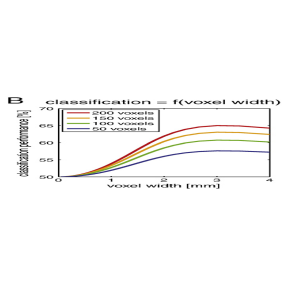
\includegraphics[height=5.5cm]{../pictures/shmuel_model}
        \end{center}
        \begin{itemize}
         \item Chaimow et al., 2010 simulated fMRI data to model decoding 
         of ODCs at different acquisition resolutions.
        \end{itemize}  
    \end{frame}

  \begin{frame}
    \frametitle{Empirical Study \textit{(under review)}}
        \begin{center}
            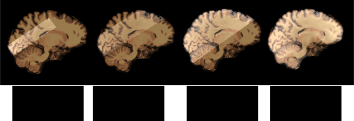
\includegraphics[height=3cm]{../pictures/acquisition}
        \end{center}
        \begin{itemize}
         \item Siemens 7 Tesla scanner with 32 channel head coil (Nova Medical, Wilmington, MA)
         \item T2*-weighted echo planar images (EPI) (TR/TE=2000/22 ms, FA=90\textdegree)
         \item Sequential acquisitions with 10\% inter-slice gap parallel to calcarine sulcus (on a tilted 
         axial plane)
        \end{itemize}  
    \end{frame}  
    
  \begin{frame}
    \frametitle{Region of interest localization}
        \begin{center}
            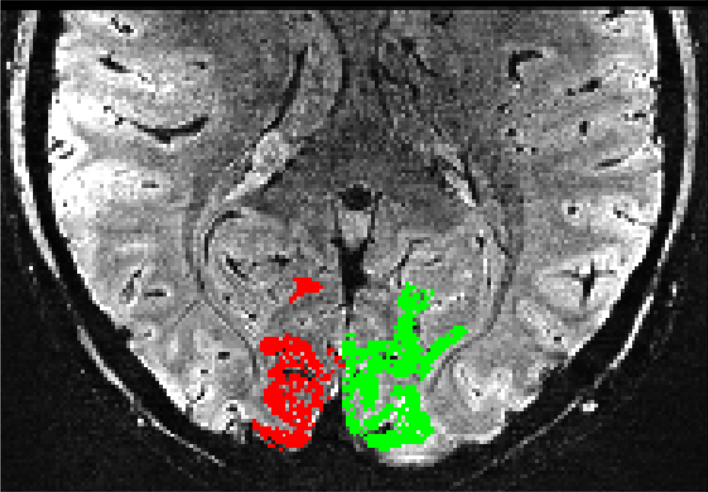
\includegraphics[height=3cm]{../pictures/ROI}
        \end{center}
                \begin{itemize}
         \item Retinotopic mapping to delineate V1 region.
         \item Susceptibility weighted imaging to localize veins.
        \end{itemize} 
    \end{frame} 
    
  \begin{frame}
    \frametitle{Classification Results (V1)}
        \begin{center}
            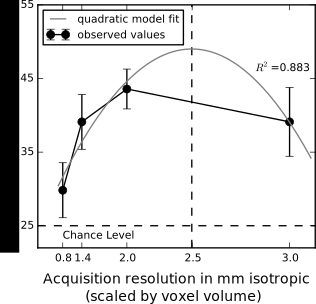
\includegraphics[height=7cm]{../pictures/classification}
        \end{center}
    \end{frame}

  \begin{frame}
        \begin{center}
            Classification / Orientation Decoding / MVPA \\ How was it performed ?
        \end{center}
    \end{frame} 

  \begin{frame}
    \frametitle{Voxel Timeseries}
        \begin{center}
            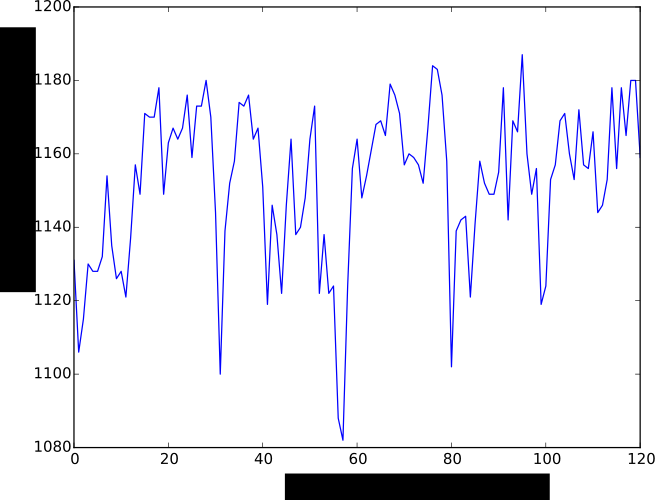
\includegraphics[height=6cm]{../pictures/time_series1}
        \end{center}
    \end{frame}

  \begin{frame}
    \frametitle{Voxel Timeseries to MVPA dataset}
        \begin{center}
            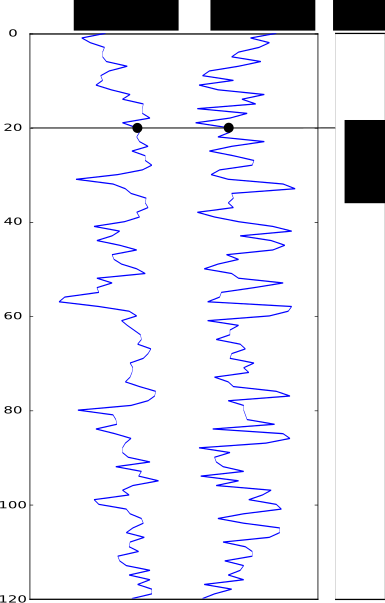
\includegraphics[height=7cm]{../pictures/time_series2dataset}
        \end{center}
    \end{frame}

  \begin{frame}
    \frametitle{MVPA dataset}
        \begin{center}
            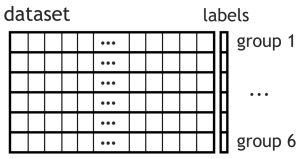
\includegraphics[height=4cm]{../pictures/mvpa_dataset}
        \end{center}
    \end{frame}

  \begin{frame}
    \frametitle{Classification Procedure}
        \begin{center}
            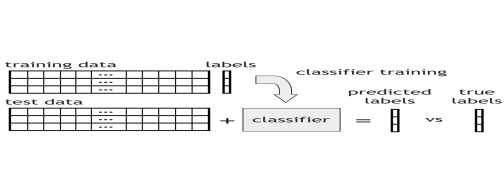
\includegraphics[height=4cm]{../pictures/classification_procedure}
        \end{center}
    \end{frame}
    
  \begin{frame}
    \frametitle{Cross Validation}
        \begin{center}
            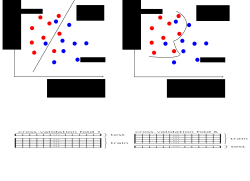
\includegraphics[height=6cm]{../pictures/cross_validation}
        \end{center}
    \end{frame}    

  \begin{frame}
    \frametitle{C parameter in LinearCSVM}
        \begin{center}
            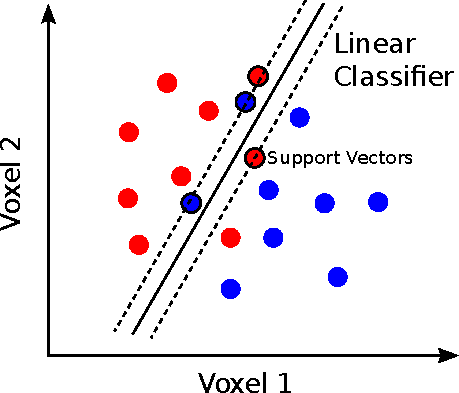
\includegraphics[height=5cm]{../pictures/margin_support_vectors}
            \begin{itemize}
             \item C parameter - Trade-off parameter between margin width and number of support vectors.
             \item Higher C – more rigid margin SVM.
            \end{itemize}  
        \end{center}     
    \end{frame}   

  \begin{frame}
    \frametitle{Nested Cross Validation}
        \begin{center}
            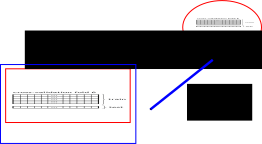
\includegraphics[height=5.5cm]{../pictures/nested_validation}
        \end{center}     
    \end{frame}  


  \begin{frame}
    \frametitle{Confusion Matrix}
        \begin{center}
            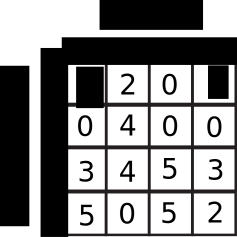
\includegraphics[height=5.5cm]{../pictures/confusion_matrix}
        \end{center}     
    \end{frame}  


  \begin{frame}
    \frametitle{Classification Results (V1)}
        \begin{center}
            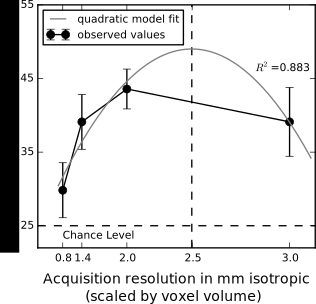
\includegraphics[height=7cm]{../pictures/classification}
        \end{center}
    \end{frame}

    
  \begin{frame}
    \frametitle{Classification Results (Fixed Number of Voxels)}
        \begin{center}
            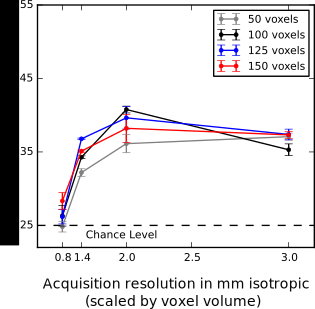
\includegraphics[height=7cm]{../pictures/fixed_voxels}
        \end{center}
    \end{frame}    

    
  \begin{frame}
    \frametitle{Classification Results after Spatial Filtering}
        \begin{center}
            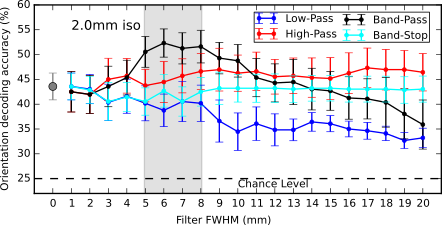
\includegraphics[height=5.5cm]{../pictures/spatial_smoothing}
        \end{center}
    \end{frame} 

  \begin{frame}
    \frametitle{Classification Results after Spatial Filtering}
        \begin{center}
            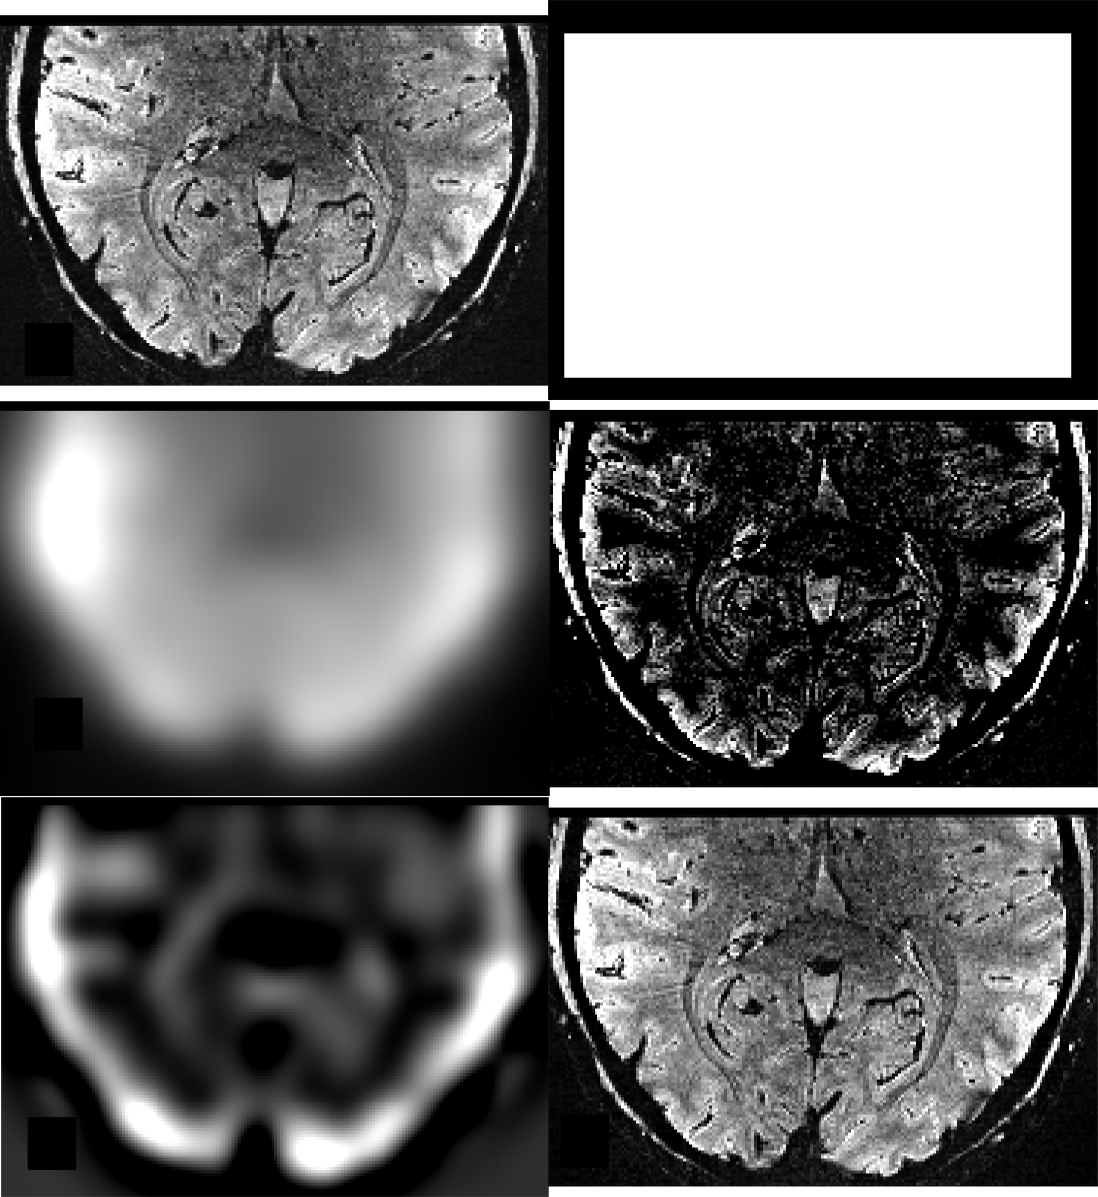
\includegraphics[height=7cm]{../pictures/filtering_steps}
        \end{center}
    \end{frame} 

  \begin{frame}
    \frametitle{Classification Results after Spatial Filtering}
        \begin{center}
            \includegraphics[height=5.5cm]{../pictures/spatial_smoothing_multires}
        \end{center}
    \end{frame} 

  \begin{frame}
    \frametitle{Contribution of veins to decoding}
        \begin{center}
            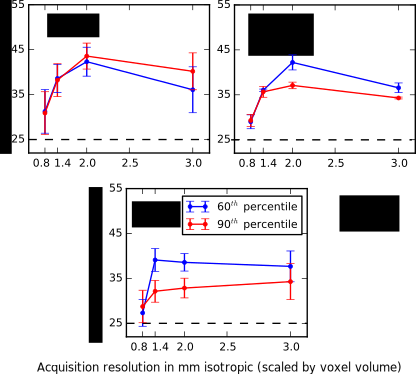
\includegraphics[height=7cm]{../pictures/veins}
        \end{center}
    \end{frame} 

  \begin{frame}
    \frametitle{Conclusions}
        \begin{center}
        \begin{itemize}
         \item Optimal Acquisition Resolution is $\approx$ 2.5mm iso.
         \item Aliasing is improbable. Highest accuracy of band-pass 
         components $\approx$ 5-8mm FWHM for all resolutions.
         \item Low spatial frequency components contribute to noise.
         %~ \item Down-sampling high resolution fMRI into lower resolutions 
         %~ does not help decoding, orientation signal not exclusively high frequency.
         \item Veins carry little orientation specific signal.
        \end{itemize}  
        \end{center}
    \end{frame} 

  \begin{frame}
    \frametitle{Acknowledgements}
        \begin{itemize}
         \item Jun. Prof. Dr. Michael Hanke
         \item Renat Yakupov
         \item Prof. Dr. Stefan Pollmann
         \item Prof. Dr. Oliver Speck
        \end{itemize}
        \vspace{1cm}
        \begin{center} 
            
\includegraphics[height=1.5cm]{../pictures/funding}
        \end{center}
    \end{frame}


  \begin{frame}
        \begin{center}
            Questions
        \end{center}
    \end{frame} 
    
  \begin{frame}
    \frametitle{Discussion: Nyquist Sampling Theory}
        \begin{center}
            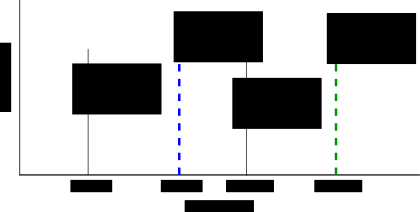
\includegraphics[height=5cm]{../pictures/nyquist}
        \end{center}
    \end{frame}                        

  \begin{frame}
    \frametitle{Discussion: Spatial smoothing does not hurt Orientation decoding}
        \begin{center}
            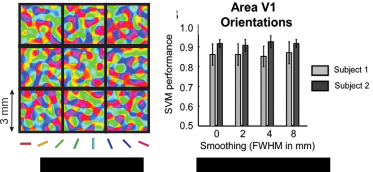
\includegraphics[height=4cm]{../pictures/grid_3mm_op_de_beeck}
        \end{center}
        \begin{itemize}
            \item Reliable Orientation decoding is possible with 3mm iso voxel size. (Kamitani and Tong, 2005 and Haynes and Rees, 2005)
            \item Above chance level decoding could be performed after spatial Gaussian smoothing.
        \end{itemize}  
    \end{frame}



  \begin{frame}
    \frametitle{Discussion: Spatial Re-sampling to Other Resolutions}
        \begin{center}
            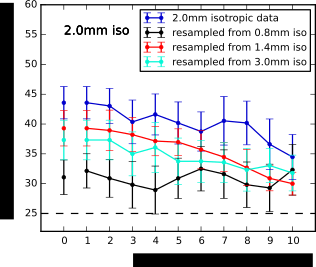
\includegraphics[height=7cm]{../pictures/resampling}
        \end{center}
    \end{frame}
    
    
  \begin{frame}
    \frametitle{Dependence on temporal SNR}
        \begin{center}
            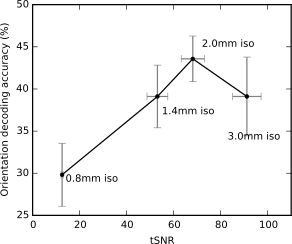
\includegraphics[height=7cm]{../pictures/tSNR_vs_accuracy}
        \end{center}
    \end{frame}    

  \begin{frame}
    \frametitle{Mean Pecrentage BOLD signal change}
        \begin{center}
            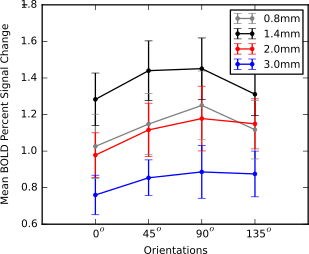
\includegraphics[height=6cm]{../pictures/signal_change}
        \end{center}
    \end{frame} 
\end{document}
   
    
